\documentclass[10pt]{beamer}

% Themes and colors for a professional look
\usetheme{Madrid}
\usecolortheme{seagull}
\setbeamercolor{title}{fg=white,bg=blue!80!black}
\setbeamercolor{frametitle}{fg=white,bg=blue!70!black}
\setbeamercolor{block title}{fg=white,bg=blue!80!black}
\setbeamercolor{block body}{bg=blue!5!white}

\title{Python Data Model}
\author{Bas Terwijn}
%\institute{\href{mailto:b.terwijn@uva.nl}{b.terwijn@uva.nl}}
\date{\today}

\begin{document}

% Title slide
\begin{frame}
    \titlepage
\end{frame}
\begin{frame}{Immutable or Mutable}
    \begin{block}{Python Types}
        Python has two different categories of types:
    \end{block}

    \vspace{1em}
    
    \textbf{Immutable Types:}
    \begin{itemize}
        \item \texttt{bool}, \texttt{int}, \texttt{float}, \texttt{complex}, \texttt{str}, \texttt{tuple}, \texttt{bytes}, \texttt{frozenset}
    \end{itemize}
    \textit{An immutable value \textbf{cannot} be modified in place. If you change it, a new copy is created.}
    
    \vspace{1em}
    
    \textbf{Mutable Types:}
    \begin{itemize}
        \item \texttt{list}, \texttt{dict}, \texttt{set}, \texttt{classes}, \dots (most other types) 
    \end{itemize}
    \textit{A mutable value \textbf{can} be modified in place.}
    
\end{frame}


\begin{frame}{Copying Mutable Values}
  When ``copying'' a \textbf{mutable} value, consider the amount of sharing you need:
    \begin{itemize}
        \item \textbf{Assignment (c1):} nothing is copied, all the values are shared
        \item \textbf{Shallow Copy (c2):} only the value referenced by the first reference is copied, all the underlying values are shared
        \item \textbf{Deep Copy (c3):} all the values are copied, nothing is shared
    \end{itemize}

    % Insert image here
    \begin{center}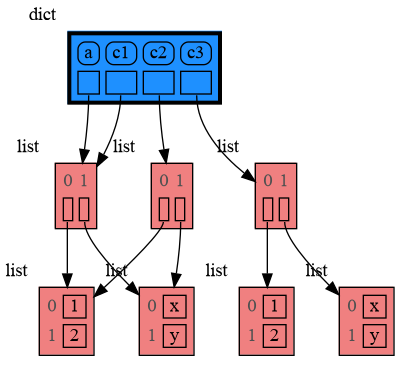
\includegraphics[width=0.4\textwidth]{figures/copy.png}\end{center}

    \begin{itemize}
        \item \textbf{Custom Copy:} write a function with your own copy logic
    \end{itemize}
\end{frame}

\begin{frame}{Function Call}
  Calling a function with a \textbf{mutable} value might change that value.
  \begin{itemize}
  \item If you don't want that, make a copy.
  \end{itemize}
  \begin{center}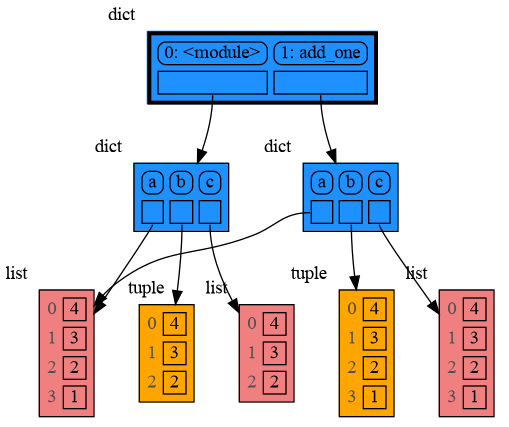
\includegraphics[width=0.6\textwidth]{figures/function_call.png}\end{center}

\end{frame}

\end{document}
